\section{Desain dan Implementasi Sistem}

\subsection{Arsitektur Sistem}
Sistem TrackMyBills terdiri dari dua komponen utama: aplikasi mobile berbasis Flutter dan backend service DonutAPI berbasis FastAPI. Arsitektur ini dipilih untuk memisahkan concern antara antarmuka pengguna dan pemrosesan model deep learning yang membutuhkan resource komputasi tinggi.

\begin{figure}[htbp]
    \centerline{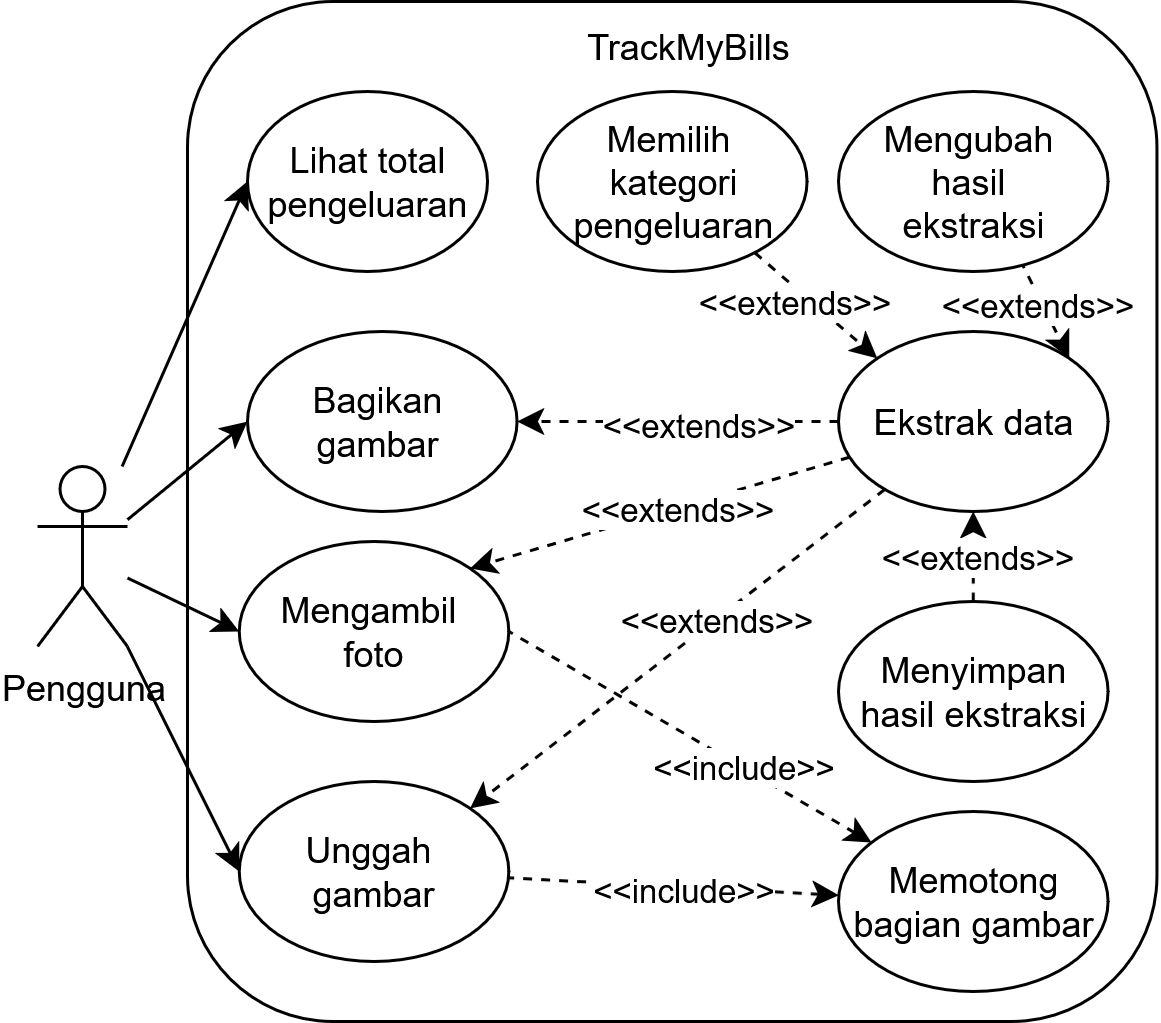
\includegraphics[width=0.45\textwidth]{images/use-case-diagram.png}}
    \caption{Use Case Diagram Sistem TrackMyBills}
    \label{fig:usecase}
\end{figure}

Gambar \ref{fig:usecase} menunjukkan use case diagram sistem yang menggambarkan interaksi pengguna dengan sistem. Pengguna dapat melakukan upload gambar bukti pembayaran, melihat hasil ekstraksi, melakukan koreksi data, dan menyimpan transaksi.

\subsection{Komponen Sistem}

\subsubsection{Aplikasi Mobile TrackMyBills}
Aplikasi mobile dikembangkan menggunakan Flutter dengan arsitektur Clean Architecture yang memisahkan layer presentation, domain, dan data. Aplikasi menyediakan antarmuka untuk:
\begin{itemize}
    \item Upload gambar dari kamera atau galeri
    \item Cropping dan preprocessing gambar
    \item Menampilkan hasil ekstraksi data
    \item Editing dan validasi data transaksi
    \item Penyimpanan lokal menggunakan SQLite
\end{itemize}

\subsubsection{Backend Service DonutAPI}
Backend service dikembangkan menggunakan FastAPI dan menyediakan endpoint REST API untuk inferensi model. Service ini mengimplementasikan dua model Donut:
\begin{itemize}
    \item \textbf{Base Model}: Fine-tuned pada dataset CORD-v2 untuk pemrosesan struk pembayaran kertas
    \item \textbf{Custom Model}: Dilatih pada dataset QRIS-TF untuk pemrosesan dokumen pembayaran digital QRIS dan transfer
\end{itemize}

\begin{figure}[htbp]
    \centerline{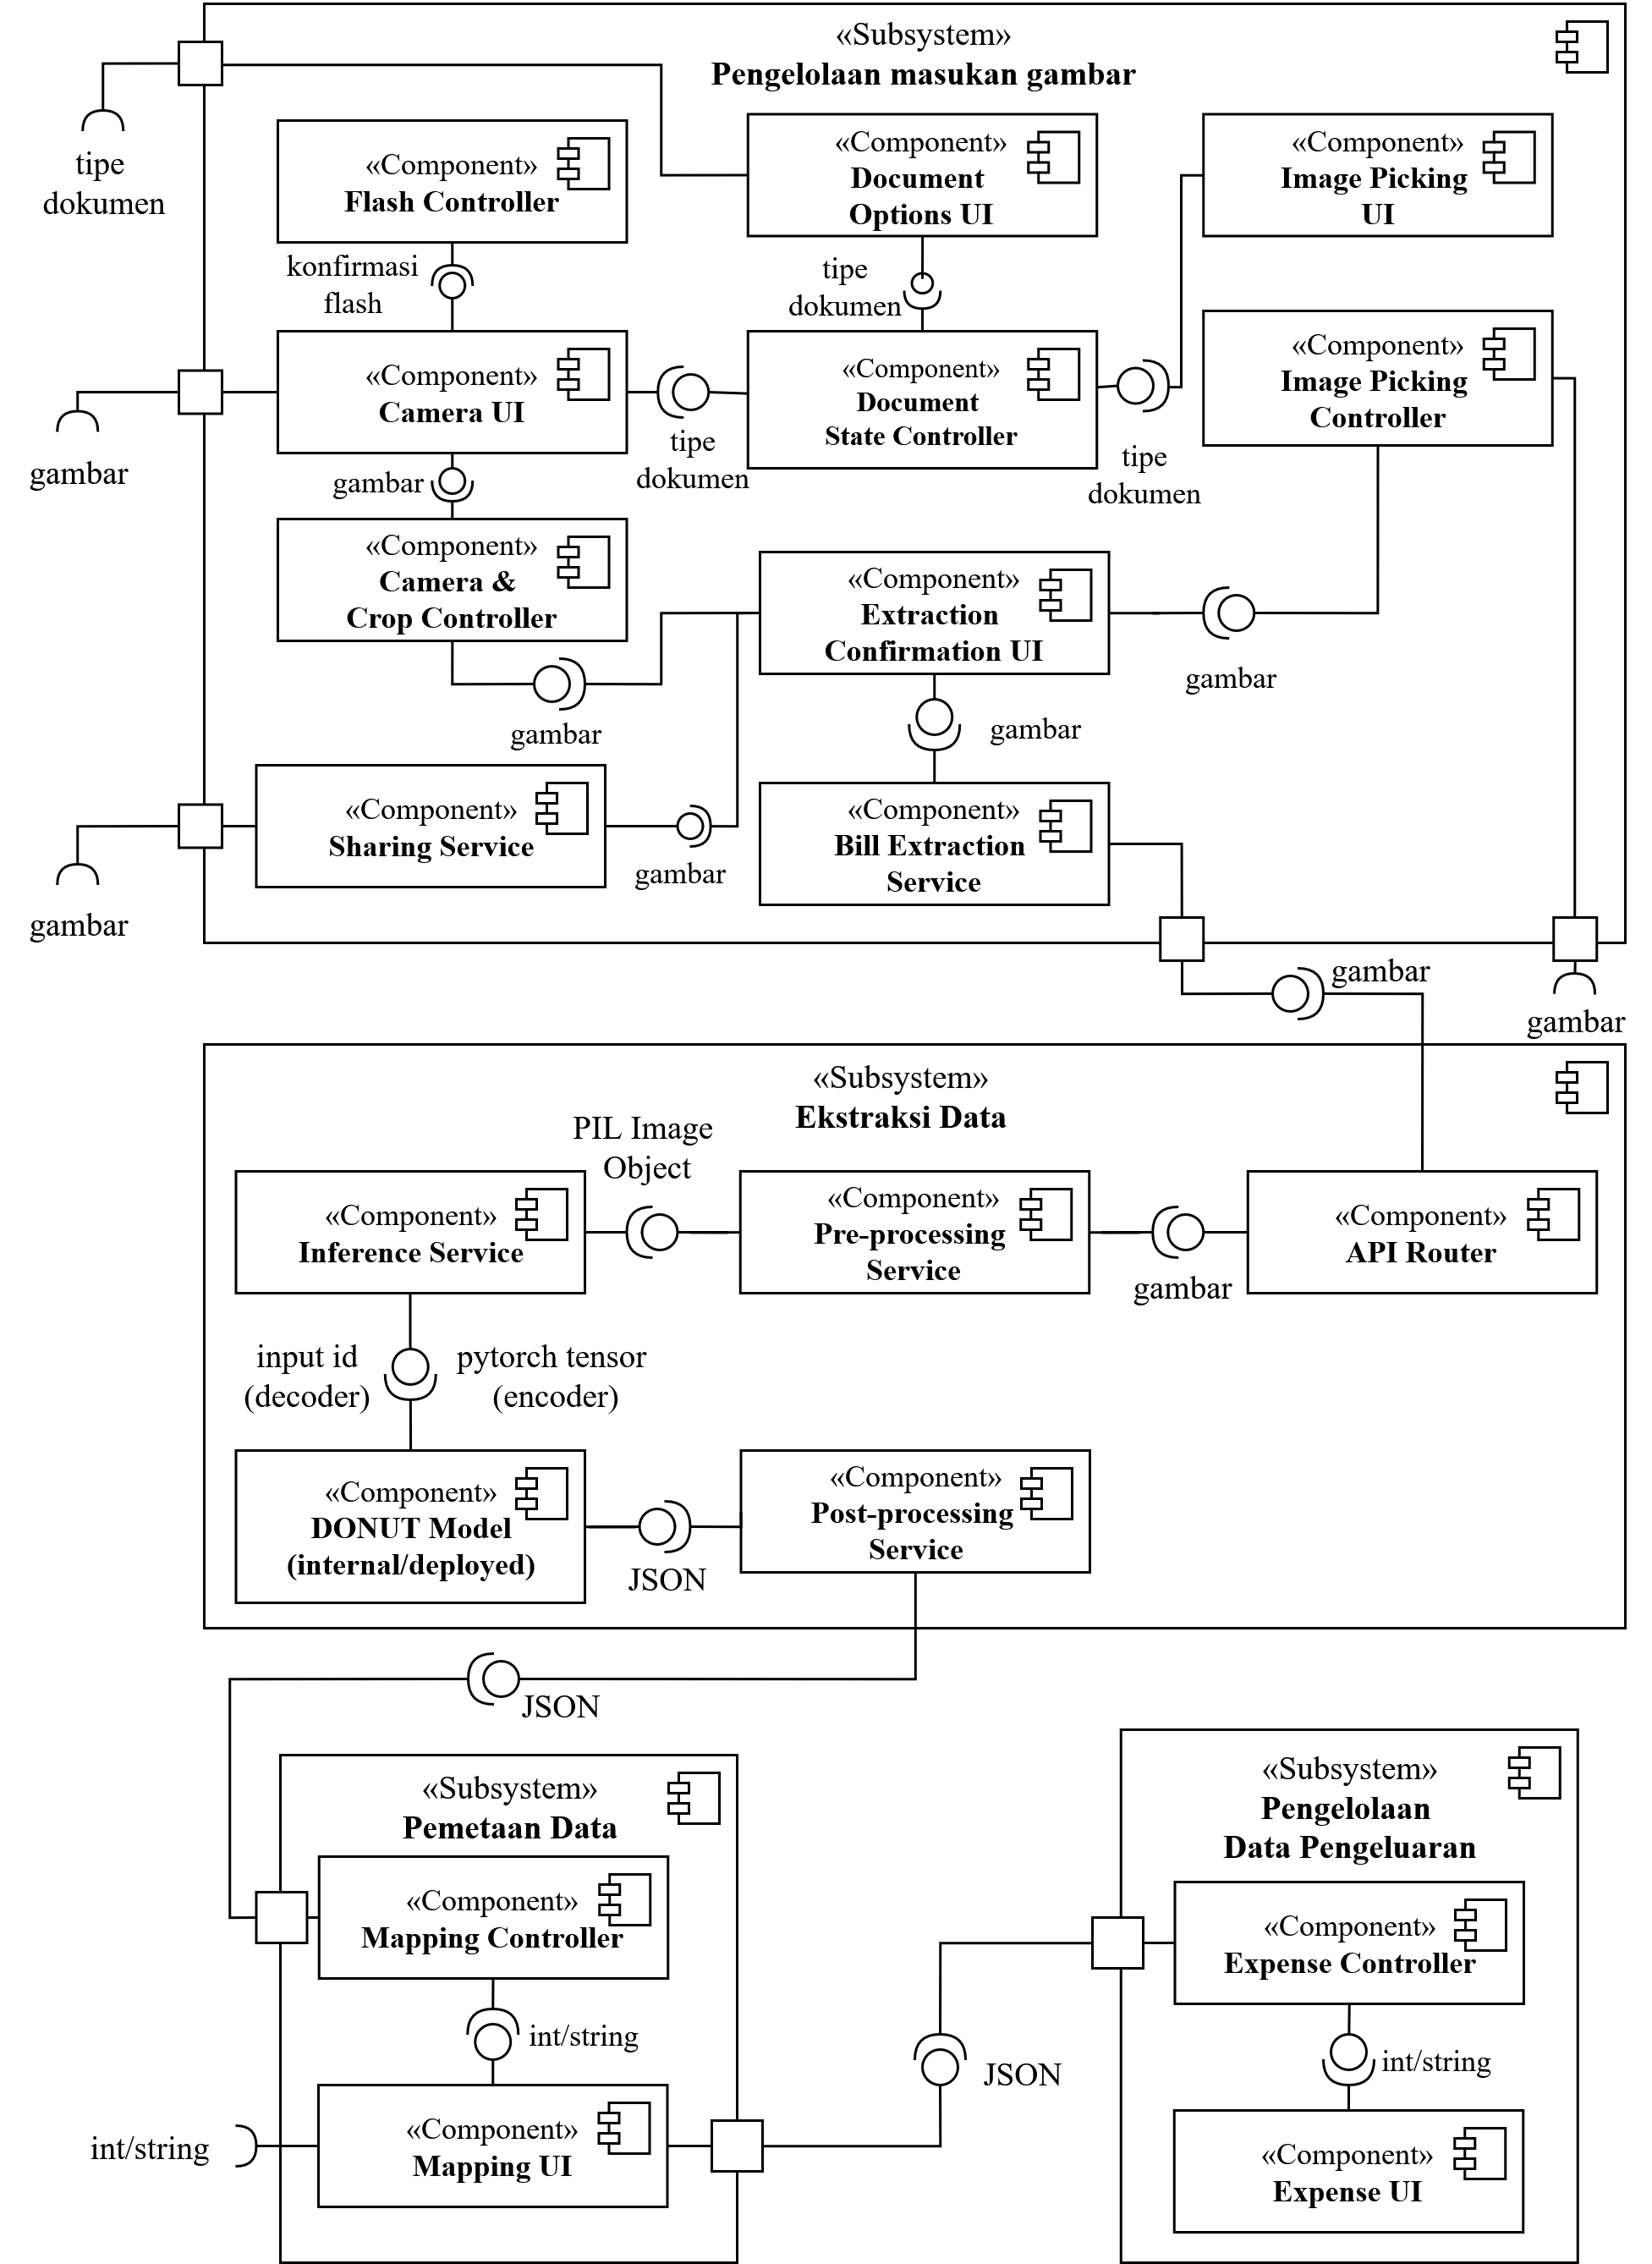
\includegraphics[width=0.45\textwidth]{images/component-diagram.png}}
    \caption{Component Diagram Sistem}
    \label{fig:component}
\end{figure}

\subsection{Pipeline Pengembangan}
\begin{figure}[htbp]
    \centerline{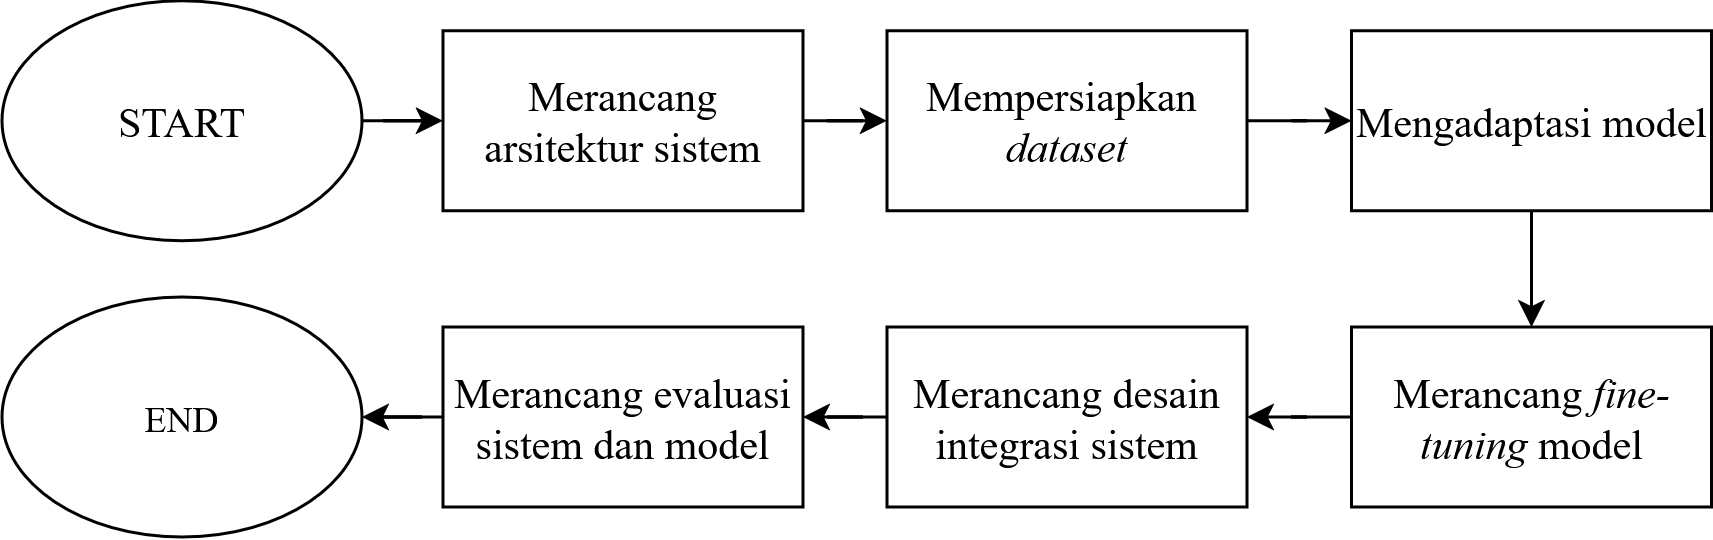
\includegraphics[width=0.45\textwidth]{images/design-flow.png}}
    \caption{Development Flow Sistem}
    \label{fig:devflow}
\end{figure}

Gambar \ref{fig:devflow} menunjukkan alur pengembangan sistem yang mengikuti metodologi Design Science Research Methodology (DSRM). Proses dimulai dari identifikasi masalah, pengumpulan dan eksplorasi data, pelatihan model, pengembangan aplikasi, hingga evaluasi sistem.

\subsection{Deployment Architecture}
\begin{figure}[htbp]
    \centerline{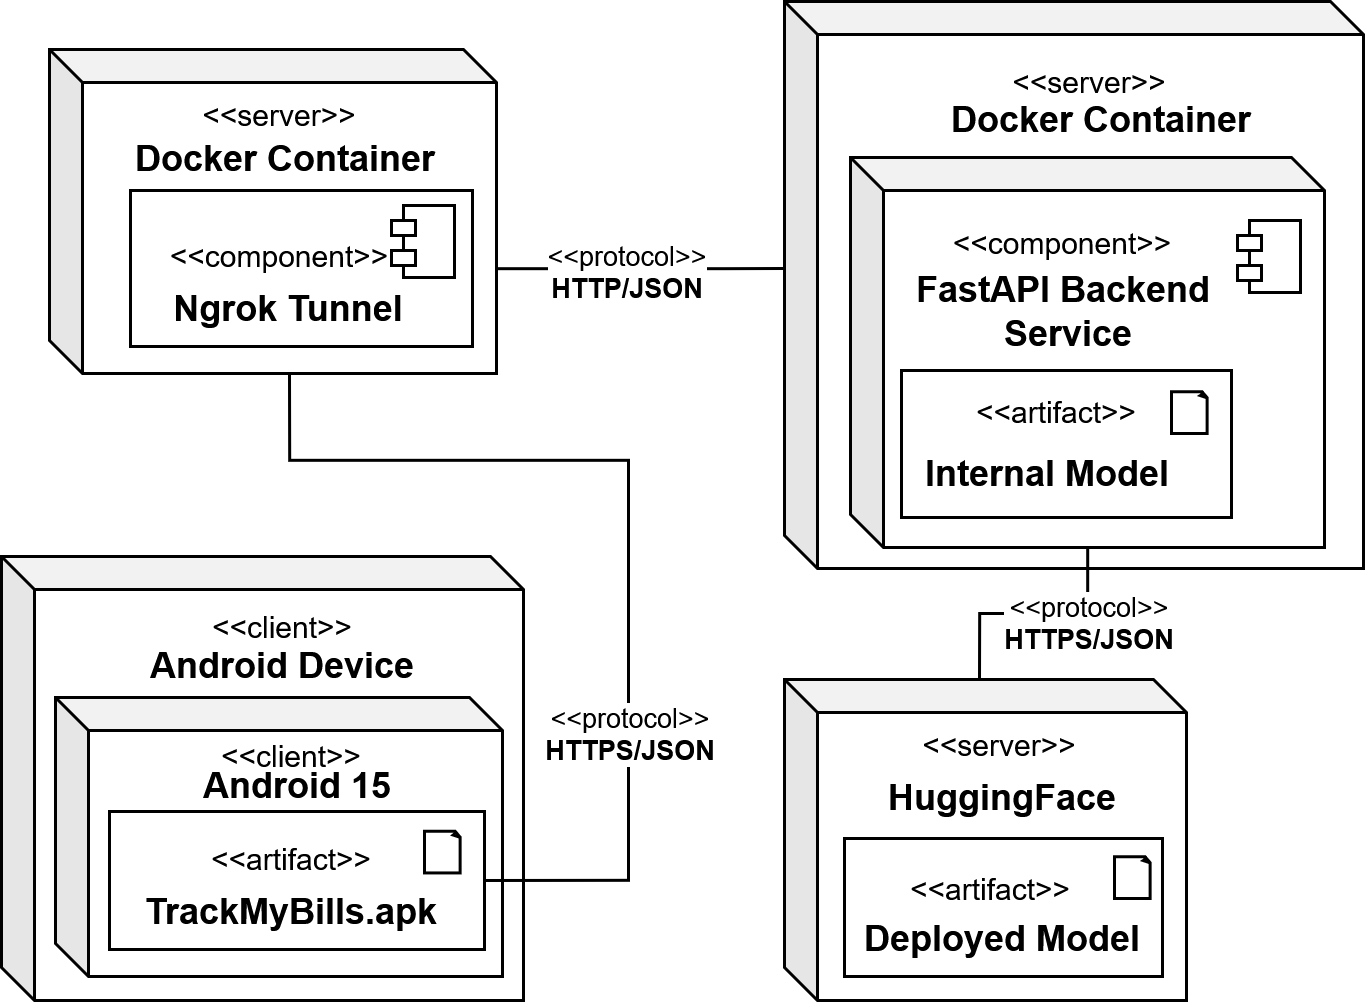
\includegraphics[width=0.45\textwidth]{images/deployment-diagram.png}}
    \caption{Deployment Diagram}
    \label{fig:deployment}
\end{figure}

Gambar \ref{fig:deployment} menggambarkan arsitektur deployment sistem. Backend service di-deploy menggunakan Docker container untuk memastikan konsistensi environment. Aplikasi mobile berkomunikasi dengan backend melalui HTTPS REST API.

\subsection{Dataset dan Preprocessing}
Penelitian ini menggunakan dua dataset utama:
\begin{itemize}
    \item \textbf{CORD-v2}: Dataset publik berisi 1,000 gambar struk pembayaran dengan anotasi terstruktur
    \item \textbf{QRIS-TF}: Dataset custom berisi 471 gambar bukti pembayaran QRIS dan transfer dari berbagai aplikasi (GoPay, SeaBank, Neobank, BCA)
\end{itemize}

Preprocessing meliputi normalisasi ukuran gambar, augmentasi data, dan konversi anotasi ke format yang kompatibel dengan model Donut. Fine-tuning dilakukan dengan learning rate 5e-5 selama 25 epoch untuk mencapai konvergensi optimal.